\chapter{Spectral methods: Galerkin and colocation}

We begin with a quote
\begin{quote}
    Spectral methods and finite-element methods are closely related and built on the same ideas; the main difference between them is that spectral methods use basis functions that are generally nonzero over the whole domain, while finite element methods use basis functions that are nonzero only on small subdomains (compact support).

    Consequently, spectral methods connect variables globally while finite elements do so locally. Partially for this reason, spectral methods have excellent error properties, with the so-called ``exponential convergence'' being the fastest possible, when the solution is smooth. However, there are no known three-dimensional single-domain spectral shock capturing results (shock waves are not smooth).

    In the finite-element community, a method where the degree of the elements is very high or increases as the grid parameter $h$ increases is sometimes called a spectral-element method.

    \url{https://en.wikipedia.org/wiki/Spectral_method}
\end{quote}

For our spectral methods we will use either Fourier basis or polynomial basis.
Within this choice of basis we will use two techniques for convergence
\begin{enumerate}
    \item Galerkin methods.

          We preserve the functional formulation of the problem (e.g., a variational equation like \eqref{eq:Galerkin elliptic variational}), but we reduce the functional space.

    \item Collocation methods

          \begin{quote}
              The idea is to choose a finite-dimensional space of candidate solutions (usually polynomials up to a certain degree) and a number of points in the domain (called collocation points), and to select that solution which satisfies the given equation at the collocation points.

              \url{https://en.wikipedia.org/wiki/Collocation_method}
          \end{quote}
\end{enumerate}

\begin{remark}
    The name \emph{spectral} makes reference to the fact that these bases are eigenfunctions (i.e., related to the \emph{spectrum}) of some differential operator: Fourier functions are eigenfunctions of the Laplacian $-\frac{d^2}{dx^2}$ and the polynomial basis we select are eigenfunctions of \emph{Sturm-Liouville} operators. But we will use to deal with general operators.
\end{remark}

\section{Colocation methods in a practical example}

\begin{example}[Colocation for the Laplace equation using Chebyshev polynomials]
    \label{ex:colocation Laplace Chebyshev}
    Consider the Laplace equation
    \begin{equation*}
        \begin{dcases}
            -\frac{d^2 u}{d x^2}(x) = f(x) & \text{for all } x \in (-1,1) \\
            u(-1) = u(1) = 0
        \end{dcases}
    \end{equation*}
    Let us look for an approximate polynomial solution $u^N \in \mathbb R^N$.
    To recover the $N+1$ coefficients uniquely we need $N+1$ independent equation.

    The colocation method consists on selecting $N+1$ points $x_0 = -1 < x_1 < \cdots < x_N = 1$ and selecting the $u^N$ such that
    \begin{equation*}
        \begin{dcases}
            -\frac{\partial^2 u^N}{\partial x^2} (x_j) = f(x_j)
             & \text{for all } j \in \{1, \cdots, N-1\} \\
            u^N(-1) = u^N(1) = 0.
        \end{dcases}
    \end{equation*}
    For each choice of $x_k$ we will be able to for $u$ expanded as combination of monomials
    \begin{equation*}
        u^N (x) = \sum_{k=0}^N c_k x^k.
    \end{equation*}

    Depending on the choice of $x_k$, it might be better to pick different basis.
    If we select as collocation points
    $x_j = \cos j \pi /N$,
    (the \emph{Chebyshev-Gauss-Lobatto} points in \Cref{ex:Chebyshev Gauss-Lobatto}),
    then it is more suitable to use the basis of Chebyshev polynomials (see \Cref{sec:Chebyshev polynomials})
    \begin{equation*}
        u^N(x) = \sum_{k=0}^N a_k T_k(x).
    \end{equation*}
    Notice by construction that $T_k (x_j) = \cos \frac{kj \pi}{N}$ because the algebraic system will be easier to write and solve.
    \begin{figure}[H]
        \centering
        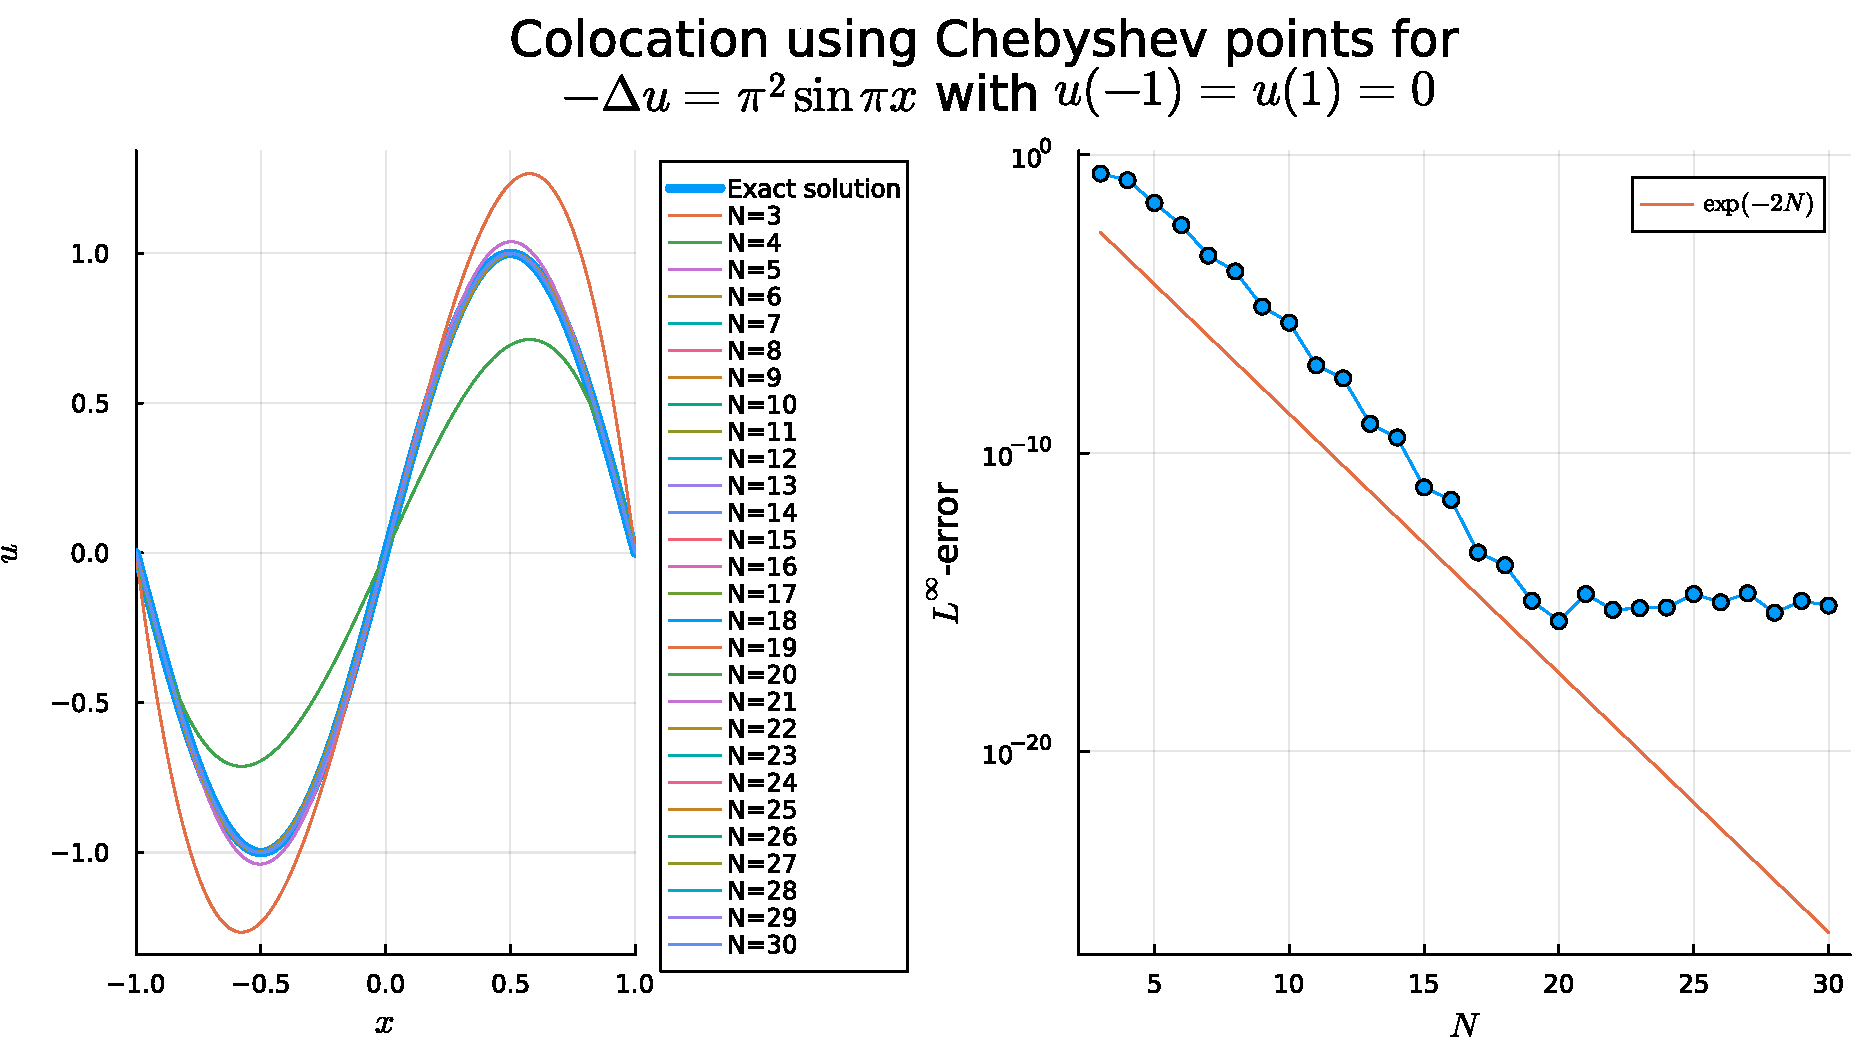
\includegraphics[width=0.75\textwidth]{convergenceChebyshev}
        \caption{Notice that the $\log \text{error} \sim -2N$ up to floating-point error. Therefore, the numerical results suggest convergence is \emph{exponential}. This very fast convergence is usually difficult to prove. A more usual result is super-polynomial convergence if $u \in C^\infty$.}
    \end{figure}
\end{example}
For the Heat Equation can follow the same reasoning to get a spacial semi-discretisation.

\bigskip

For the remaining Chapters we will follow essentially \cite{CanutoHussainiQuarteroniZang2011}.

\section{Linear algebra representation of spectral colocation methods}
\label{sec:spectral colocation linear algebra}

Given a basis $\phi_k$ such that ``reasonable'' functions can be expressed as for some set $Z \subset \mathbb Z$ for a large enough class of functions $v \in V$
\begin{equation*}
    v(x) = \sum_{k \in Z} \hat v_k \phi_k(x)
\end{equation*}
Then we take a finite set $Z_N = \{k_0, \cdots, k_N\} \subset Z$ and we look for solutions
\begin{equation*}
    u_N(x) = \sum_{k \in Z_N} \hat u_k \phi_k(x)
\end{equation*}
Let $V_N$ be the set of space of such functions.

\bigskip

Galerkin's method usually lead to equation on the terms $\hat u_k$. However, colocation methods of points $x_0, \cdots, x_N$ are written in terms of the value $u_N(t,x_j)$.
Let us write this in matrix form as
\begin{equation*}
    u_N(x)
    = (\phi_{k_0} (x), \cdots, \phi_{k_N}(x))
    \vec {\hat u}_N,
    \qquad \text{where }\vec{\hat u}_N
    =
    \begin{pmatrix}
        \hat u_{k_0} \\ \vdots \\ \hat u_{k_N}
    \end{pmatrix}.
\end{equation*}
and so we can write a system of linear relations between $\widehat u_{k}$ and $u_N (x_i)$
\begin{equation*}
    \begin{pmatrix}
        u_N(x_0) \\ \vdots \\ u_N(x_N)
    \end{pmatrix}
    =
    \underbrace{
        \begin{pmatrix}
            \phi_{k_0} (x_0) & \cdots & \phi_{k_N}(x_0) \\
                             & \vdots                   \\
            \phi_{k_0} (x_N) & \cdots & \phi_{k_N}(x_N) \\
        \end{pmatrix}
    }_{\mat A_N}
    \vec{\hat u}_N,
\end{equation*}

In the spectral basis we will use we have that $\frac{\partial \phi_k}{\partial x} \in V_N$ if $k \le N$. Hence we can write
\begin{equation*}
    \begin{pmatrix}
        \frac{d \phi_{k_0}}{d x} (x)
        \\
        \vdots \\
        \frac{d \phi_{k_N}}{d x} (x)
    \end{pmatrix}
    = \mat B_N^t
    \begin{pmatrix}
        \phi_{k_0} (x) \\ \vdots \\ \phi_{k_N}(x)
    \end{pmatrix},
\end{equation*}
and hence
\begin{equation*}
    \frac{d u_N}{d x} (x)
    =  \left(\frac{d \phi_{k_0}}{d x} (x), \cdots, \frac{d \phi_{k_N}}{d x}\right)
    \vec{\hat u}_N
    = (\phi_{k_0} (x), \cdots, \phi_{k_N}(x)) \mat D_N^t \vec {\hat u}_N.
\end{equation*}
Then we have that
\begin{equation*}
    \begin{pmatrix}
        \frac{d u_N}{dx}(x_0) \\ \vdots \\ \frac{d u_N}{dx} (x_N).
    \end{pmatrix}
    =
    \underbrace{\mat A_N \mat B_N \mat A_N^{-1}}_{\mat D_N}
    \begin{pmatrix}
        u_N(x_0) \\ \vdots \\ u_N(x_N)
    \end{pmatrix}.
\end{equation*}
We can iterate this process to deduce that
\begin{equation*}
    \begin{pmatrix}
        \frac{d^2 u_N}{dx^2}(x_0) \\ \vdots \\ \frac{d^2 u_N}{dx^2} (x_N).
    \end{pmatrix}
    =
    \mat D_N^2
    \begin{pmatrix}
        u_N(x_0) \\ \vdots \\ u_N(x_N)
    \end{pmatrix}.
\end{equation*}


If the basis $\phi_k$ is orthogonal in some scalar product, the elements of $\mat B_N$ are easy to compute.


\begin{remark}
    \label{rem:pointwise evaluation plotting}
    Pointwise evaluations are suitable for plotting. However, if we wanted to recover the basis coefficients we can use $\mat A_N$.
\end{remark}